\chapter{航天器姿态运动学}
\thispagestyle{empty}

\section{航天器常用坐标系}
\subsection{基本概念}
\vspace*{-1em}

\defination[天体坐标系基本概念]
{
	\dy[天球]{{\text{T}}Q}\quad 指一个以地球质心$M$为中心,半径$r$为任意长的一个假想的球体 。其目的是将天体沿观测者视线投影到球面上,以便于研究天体及其相互关系。\\
	\hspace*{2.2em}\dy[黄道平面]{HDPM}\quad 由于地球绕太阳公公转而产生的,即地球公转轨道在天球上的反映称为黄道。它和赤道面相交于春分点和秋分点。\\
	\hspace*{2.2em}\dy[春分点]{CFD}\quad 指太阳从难向北在黄赤道上的交点。
}

\begin{figure}[!htb]
	\begin{minipage}{0.45\linewidth}
		\centering
		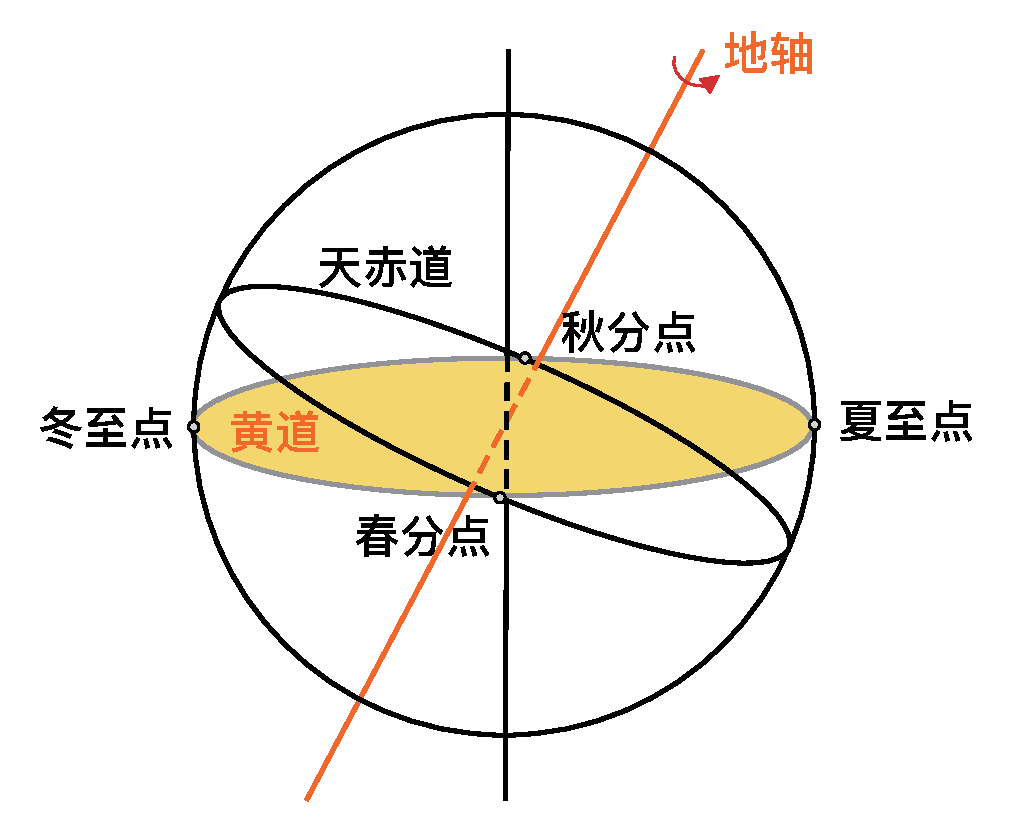
\includegraphics[width=\linewidth]{pic/基本概念}
		\caption{天球坐标系的基本概念}
		\label{基本概念}
	\end{minipage}
	\begin{minipage}{0.55\linewidth}
		\centering
		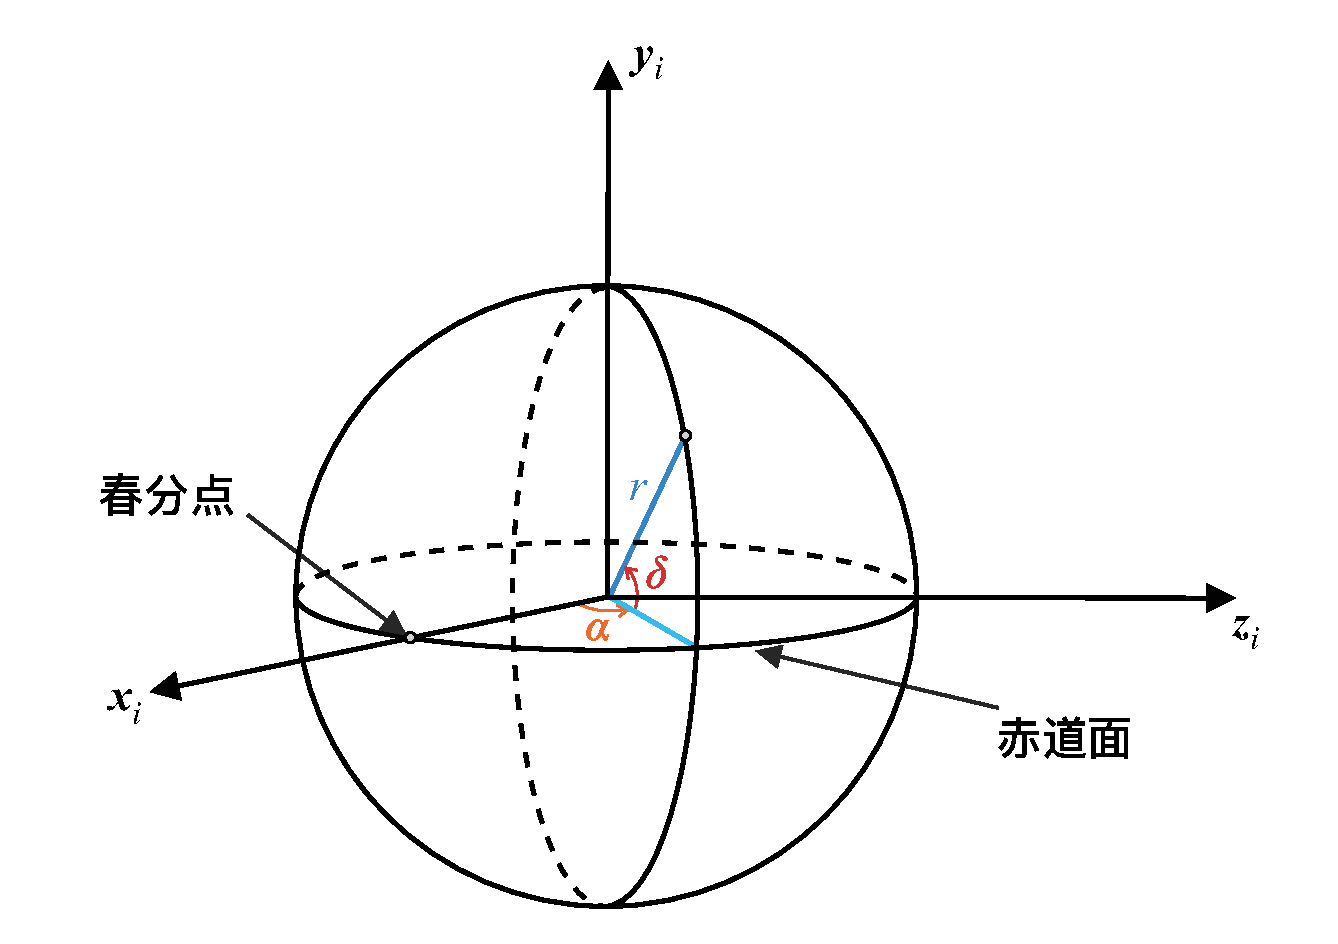
\includegraphics[width=\linewidth]{pic/地惯}
		\vspace*{-2.9em}
		\caption{地心赤道惯性坐标系}
		\label{地惯}
	\end{minipage}
\end{figure}


\subsection{地心赤道惯性坐标系}
\vspace*{-1em}

\defination[地心赤道惯性坐标系]
{
	如图 \ref{地惯} 所示,\dy[地心第一赤道坐标系]{DXDYCDZBX},简称为\dy[惯性坐标系]{GXZBX}。$X$轴在地球赤道平面内,指向赤道平面与黄道平面的相交线交点(春分点)。$Z$轴垂直于赤道平面,与地球自转角速度矢量方向一致。J2000的地心平赤道、平春分点的地心赤道坐标系。
}


\subsection{地心赤道旋转坐标系}
\vspace*{-1em}

\defination[地心赤道坐标系]
{
	如图 \ref{地心旋转} 所示,\dy[地心赤道旋转坐标系]{DXCDXZZBX},也叫\dy[地心第四赤道坐标系]{DXDSCDZBX}。$X$轴在赤道平面内,指向\dy[格林威治子午线]{GLNZZWX},$Z$轴垂直于赤道平面,与地球自转角速度矢量方向一致。$\lambda$是地理经度,从格林威治子午线向东度量,$\phi$是地心纬度。
}

\begin{figure}[!htb]
	\begin{minipage}{0.485\linewidth}
		\centering
		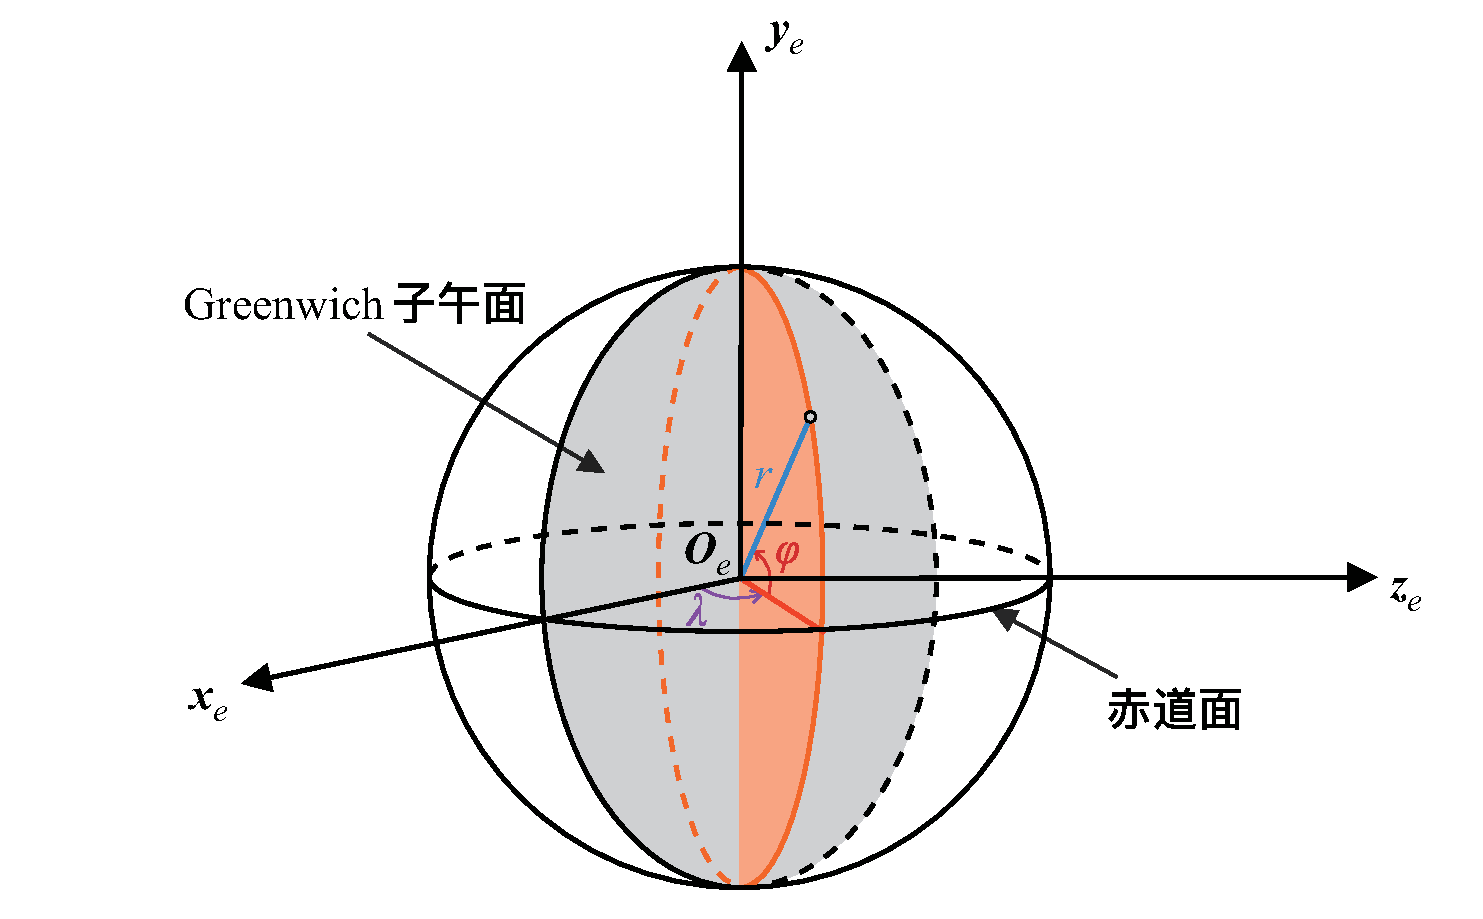
\includegraphics[width=\linewidth]{pic/地心旋转}
		\caption{地心赤道旋转坐标系}
		\label{地心旋转}
	\end{minipage}
	\begin{minipage}{0.515\linewidth}
		\centering
		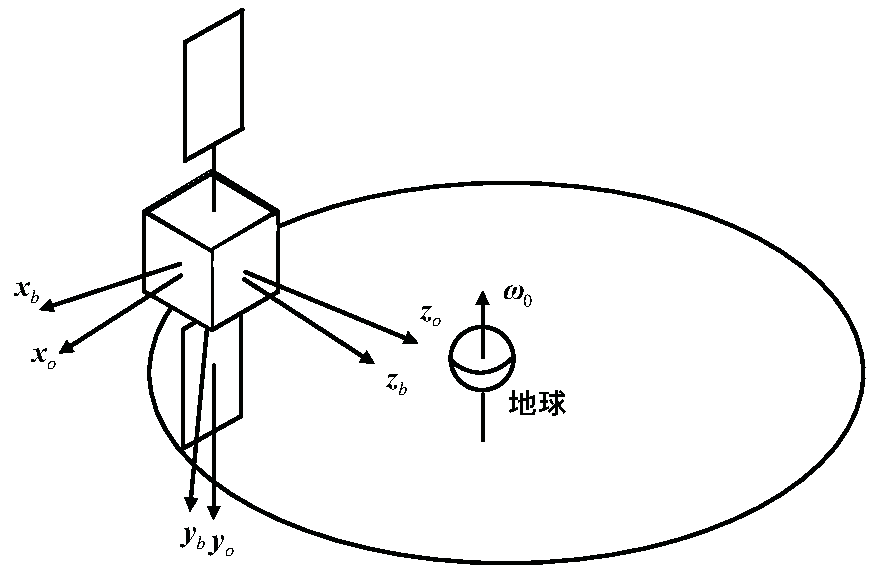
\includegraphics[width=\linewidth]{pic/轨道星体}
		\caption{轨道坐标系和星体坐标系}
		\label{轨道星体}
	\end{minipage}
\end{figure}


\subsection{轨道坐标系和星体坐标系}
\vspace*{-1em}

\defination[地心赤道坐标系]
{
	\dy[轨道坐标系]{DY}\quad 原点在飞行器质心,$z_o$轴指向地心,$x_o$轴在轨道面内与$z_o$轴垂直,指向速度方向,$y_o$轴在轨道平面法线方向,与$x_o$,$z_o$轴成右手正交坐标系。\\
	\hspace*{2.2em}\dy[星体坐标系]{X{\text{T}}ZBX}\quad 原点在质心,$x_b$轴为\dy[滚动轴]{GDZ},$y_b$轴为\dy[俯仰轴]{FYZ},$z_b$轴为\dy[偏航轴]{PHZ}。(对地定向航天器)
}


\section{姿态参数}
\subsection{方向余弦矩阵}
	对于坐标系原点重合的两个不同的坐标系$S_a$和$S_b$,坐标基分别为$\bm{e}_a$和$\bm{e}$
,对于矢量$\bm{u}$在两个坐标系下的分解,有
\begin{equation}
	\bm{u} = \bm{e}_b^{\text{T}}u_b = \bm{e}_a^{\text{T}}u_a
\end{equation}
两边同时乘以$\bm{e}_b$,得
\begin{equation*}
	\bm{e}_b \bm{e}_b^{\text{T}} u_b = \bm{e}_b \bm{e}_a^{\text{T}} u_a \quad \Rightarrow \quad u_b = \bm{e}_b\bm{e}_au_a^{\text{T}}
\end{equation*}
为此我们定义坐标系$S_a$变换为坐标系$S_b$的\dy[方向余弦矩阵]{FXYXJZ}为
\begin{equation}
	\bm{C}_{ba} = \bm{e}_b \bm{e}_a^{\text{T}}
	=
	\begin{bmatrix}
		\bm{i}_b \cdot \bm{e}_a^{\text{T}} \\
		\bm{j}_b \cdot \bm{e}_a^{\text{T}} \\
		\bm{k}_b \cdot \bm{e}_a^{\text{T}} 
	\end{bmatrix}
	=
	\begin{bmatrix}
		\bm{i}_b \cdot \bm{i}_a & \bm{i}_b \cdot \bm{j}_a & \bm{i}_b \cdot \bm{k}_a \\
		\bm{j}_b \cdot  \bm{i}_a & \bm{j}_b \cdot \bm{j}_a & \bm{j}_b \cdot \bm{k}_a \\
		\bm{k}_b \cdot  \bm{i}_a & \bm{k}_b \cdot \bm{j}_a & \bm{k}_b \cdot \bm{k}_a 
	\end{bmatrix}
	=
	\begin{bmatrix}
		C_{11} & C_{12} & C_{13} \\
		C_{21} & C_{22} & C_{23} \\
		C_{31} & C_{32} & C_{33}
	\end{bmatrix}
\end{equation}
方向余弦矩阵有以下几个特征:

\newpage

\sssection[6个约束方程]
\noa[1] 模值约束
\begin{equation}
	\begin{cases}
		\,\big|\bm{i}_b\big|^2 = C_{11}^2 + C_{12}^2 + C_{13}^2 = 1\\
		\,\big|\bm{j}_b\big|^2 = C_{21}^2 + C_{22}^2 + C_{23}^2 = 1\\
		\,\big|\bm{k}_b\big|^2 = C_{31}^2 + C_{32}^2 + C_{33}^2 = 1
	\end{cases}
\end{equation}
\proof 由于$\bm{i}_b, \bm{j}_b, \bm{k}_b$的模值为1(空间绝对),所以将它们投影到坐标系$S_a$后模值仍然为1,即
\begin{equation*}
	\begin{cases}
		\,\big|\bm{i}_b \cdot \bm{e}_a^{\text{T}}\big|^2 = \big|\bm{i}_b\big|^2 = 1\\
		\,\big|\bm{j}_b \cdot \bm{e}_a^{\text{T}}\big|^2 = \big|\bm{j}_b\big|^2 = 1\\
		\,\big|\bm{k}_b \cdot \bm{e}_a^{\text{T}}\big|^2 = \big|\bm{k}_b\big|^2 = 1\\
	\end{cases}
	\qquad \Longrightarrow \qquad 
	\begin{cases}
		\,\big|\bm{i}_b\big|^2 = C_{11}^2 + C_{12}^2 + C_{13}^2 = 1\\
		\,\big|\bm{j}_b\big|^2 = C_{21}^2 + C_{22}^2 + C_{23}^2 = 1\\
		\,\big|\bm{k}_b\big|^2 = C_{31}^2 + C_{32}^2 + C_{33}^2 = 1
	\end{cases}
\end{equation*}

\noa[2] 几何约束
\begin{equation}
	\begin{cases}
		\,\bm{i}_b \cdot \bm{j}_b = C_{11}C_{21} + C_{12}C_{22} + C_{13}C_{23} = 0 \\
		\,\bm{i}_b \cdot \bm{k}_b = C_{11}C_{31} + C_{12}C_{32} + C_{13}C_{33} = 0 \\
		\,\bm{j}_b \cdot \bm{k}_b = C_{21}C_{31} + C_{22}C_{32} + C_{23}C_{33} = 0
	\end{cases}
\end{equation}
\proof 由于$\bm{i}_b, \bm{j}_b, \bm{k}_b$两两正交(空间绝对),所以将它们投影到坐标系$S_a$后仍然满足几何关系,即
\begin{equation*}
	\begin{cases}
		\,\bm{i}_b \cdot \bm{j}_b = \big(\bm{i}_b \cdot \bm{e}_a^{\text{T}}\big) \cdot  \big(\bm{j}_b \cdot \bm{e}_a^{\text{T}}\big) = 0\\
		\,\bm{i}_b \cdot \bm{k}_b = \big(\bm{i}_b \cdot \bm{e}_a^{\text{T}}\big) \cdot \big(\bm{k}_b \cdot \bm{e}_a^{\text{T}}\big) = 0\\
		\,\bm{j}_b \cdot \bm{k}_b =\big(\bm{j}_b \cdot \bm{e}_a^{\text{T}}\big) \cdot \big(\bm{k}_b \cdot \bm{e}_a^{\text{T}}\big) = 0
	\end{cases}
	\qquad \Longrightarrow \qquad 
	\begin{cases}
		\,\bm{i}_b \cdot \bm{j}_b = C_{11}C_{21} + C_{12}C_{22} + C_{13}C_{23} = 0 \\
		\,\bm{i}_b \cdot \bm{k}_b = C_{11}C_{31} + C_{12}C_{32} + C_{13}C_{33} = 0 \\
		\,\bm{j}_b \cdot \bm{k}_b = C_{21}C_{31} + C_{22}C_{32} + C_{23}C_{33} = 0
	\end{cases}
\end{equation*}


\vspace*{0.5em}
\sssection[坐标变换矩阵是正交矩阵]

由于
\begin{equation*}
	\begin{cases}
		\,\bm{e}_b \cdot \bm{e}_b^{\text{T}} = \bm{e}_a \cdot \bm{e}_a^{\text{T}} = \bm{E}_3\\
		\,\bm{e}_b \cdot \bm{e}_b^{\text{T}} = \bm{C}_{ba}\bm{e}_a \cdot \big( \bm{C}_{ba} \bm{e}_a \big)^{\text{T}} =  \bm{C}_{ba}\bm{e}_a \cdot \bm{e}_a^{\text{T}} \bm{C}_{ba}^{\text{T}} 
	\end{cases}
	\quad \Rightarrow \quad \bm{E}_3 = \bm{C}_{ba} \cdot \big( \bm{e}_a \cdot \bm{e}_a^{\text{T}} \big) \cdot \bm{C}_{ba}^{\text{T}} =  \bm{C}_{ba} \cdot \bm{C}_{ba}^{\text{T}}
\end{equation*}
所以可以得到
\begin{equation}
	\bm{C}_{ba}^{\text{T}} = \bm{C}_{ba}^{-1}
\end{equation}
且有
\begin{equation}
	\bm{C}_{ab} = \bm{e}_a \cdot \bm{e}_b^{\text{T}} = \bm{e}_a \cdot \bm{e}_a^{\text{T}} \bm{C}_{ba}^{\text{T}} = \bm{C}_{ba}^{-1}
\end{equation}


\vspace*{0.5em}
\sssection[坐标变换矩阵的行列式为1]

由于矩阵乘积的行列式等于行列式的乘积且矩阵的转置的行列式等于矩阵的行列式,所以
\begin{equation}
	\det \big(\bm{C}_{ba}\big) \det \big(\bm{C}_{ba}^{\text{T}}\big) 
	= \big[ \det \big(\bm{C}_{ba} \big) \big]^2 
	= \det \big( \bm{C}_{ba} \cdot \bm{C}_{ba}^{\text{T}} \big) 
	= 1
	\quad \Rightarrow \quad 
	\det \big(\bm{C}_{ba}\big) = \pm 1
\end{equation}
而因为
\begin{equation*}
	\bm{C}_{ba}^{\text{T}} = \text{adj}\big( \bm{C}_{ba} \big) 
	\quad  \Rightarrow \quad 
	\bm{C}_{ba}^{-1} 
	= \dfrac{\text{adj}\big( \bm{C}_{ba} \big)}{\det \big( \bm{C}_{ba} \big)} 
	= \dfrac{\bm{C}_{ba}^{\text{T}}}{\det \big( \bm{C}_{ba} \big)} 
	= \dfrac{\bm{C}_{ba}^{-1}}{\det \big( \bm{C}_{ba} \big)}
\end{equation*}
因此
\begin{equation}
	\det \big( \bm{C}_{ba} \big) = + 1
\end{equation}

\clearpage


\sssection[相继运动的坐标变换矩阵]

对于坐标系原点重合的三个不同的坐标系$S_a$,$S_b$和$S_c$,有
\begin{equation*}
	\begin{cases}
		\, \bm{e}_b \cdot \bm{e}_a^{\text{T}} = \bm{C}_{ba} \\
		\, \bm{e}_c \cdot \bm{e}_b^{\text{T}} = \bm{C}_{cb} \\
		\, \bm{e}_c \cdot \bm{e}_a^{\text{T}} = \bm{C}_{ca}
	\end{cases}
	\quad \Rightarrow \quad 
	\bm{e}_c = \bm{C}_{ca} \bm{e}_a = \bm{C}_{cb}\bm{e}_b = \bm{C}_{cb} \bm{C}_{ba} \bm{e}_{a}
\end{equation*}
因此
\begin{equation}
	\bm{C}_{ca} = \bm{C}_{cb} \bm{C}_{ba}
\end{equation}
\vspace*{0.5em}


\subsection{欧拉角}
\vspace*{-1em}

\defination[基元旋转矩阵]
{
	\dy[基元旋转矩阵]{JYXZJZ}\quad 任何一个坐标变换可以看成是绕三个基本轴的旋转,这三个基本轴的坐标转换矩阵为基元旋转矩阵,如图 \ref{x}, \ref{y}, \ref{z} 所示,绕各个轴旋转的角度称为\dy[欧拉角]{OLJ}。每个坐标轴对应的基元旋转矩阵为
	\begin{equation}
		\bm{C}_x (\varphi) =
		\begin{bmatrix}
			1 & 0 & 0 \\
			0 & \cos \varphi & \sin \varphi \\
			0 & - \sin \varphi & \cos \varphi 
		\end{bmatrix}
		\qquad \quad
		\bm{C}_y (\theta) = 
		\begin{bmatrix}
			\cos \theta & 0 & - \sin \theta \\
			0 & 1 & 0 \\
			\sin \theta & 0 & \sin \theta 
		\end{bmatrix}
		\qquad \quad
		\bm{C}_z (\psi) = 
		\begin{bmatrix}
			\cos \psi & \sin \psi & 0 \\
			- \sin \psi &\cos \psi & 0 \\
			0 & 0 & 1
		\end{bmatrix}
	\end{equation}
	{	
		\centering
		\begin{minipage}{0.34\linewidth}
			\centering
			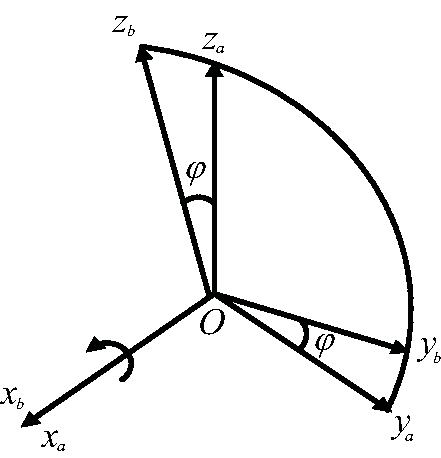
\includegraphics[width=0.77\linewidth]{pic/x}
			\vspace*{-0.5em}
			\captionof{figure}{绕$x$轴旋转}
			\label{x}
		\end{minipage}
		\begin{minipage}{0.3\linewidth}
			\centering
			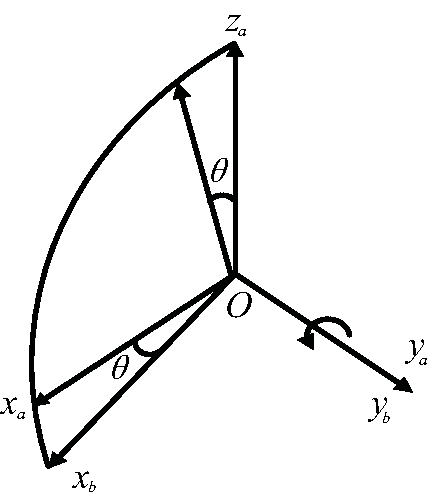
\includegraphics[width=0.78\linewidth]{pic/y}
			\vspace*{-0.5em}
			\captionof{figure}{绕$y$轴旋转}
			\label{y}
		\end{minipage}
		\begin{minipage}{0.34\linewidth}
			\centering
			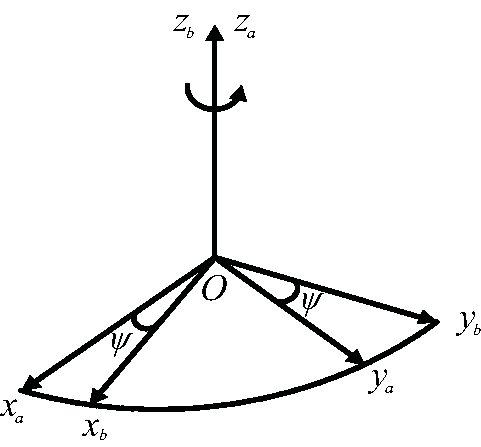
\includegraphics[width=0.85\linewidth]{pic/z}
			\vspace*{-0.5em}
			\captionof{figure}{绕$z$轴旋转}
			\label{z}
		\end{minipage}
	}
}

下面给出两种基元旋转矩阵表示的坐标变换。
\vspace*{0.5em}

\sssection[$ZXZ$旋转顺序]

如图 \ref{ZXZ} 所示,方向余弦矩阵和$ZXZ$顺序欧拉角的关系为
\begin{equation}
	\bm{C}_{ba} = \bm{C}_z(\varphi) \bm{C}_x(\theta) \bm{C}_z(\psi) = 
	\begin{bmatrix}
		\cos \varphi \cos \psi - \sin \varphi \cos \theta \sin \psi & \cos \varpi \sin \psi + \sin \varphi \cos \theta \cos \psi & \sin \varphi \sin \theta \\
		- \sin \varphi \cos \psi - \cos \varphi \cos \theta \sin \psi & -\sin \varphi \sin \psi + \cos \varphi \cos \theta \cos \psi & \cos \varphi \sin \theta \\
		\sin \theta \sin \psi & -\sin \theta \cos \psi & \cos \theta 
	\end{bmatrix}
\end{equation}
通过与方向余弦矩阵的对应项进行对比,可以计算得到
\begin{equation}
	\begin{cases}
		\, \psi = -\tan^{-1}\left( \dfrac{C_{31}}{C_{32}} \right) \\
		\, \theta = \cos^{-1}\big( C_{33} \big) \\
		\, \varphi = \tan^{-1} \left( \dfrac{C_{13}}{C_{23}} \right)
	\end{cases}
	\label{eq:zxz}
\end{equation}
\clearpage

\begin{figure}[!htb]
	\begin{minipage}{0.5\linewidth}
		\centering
		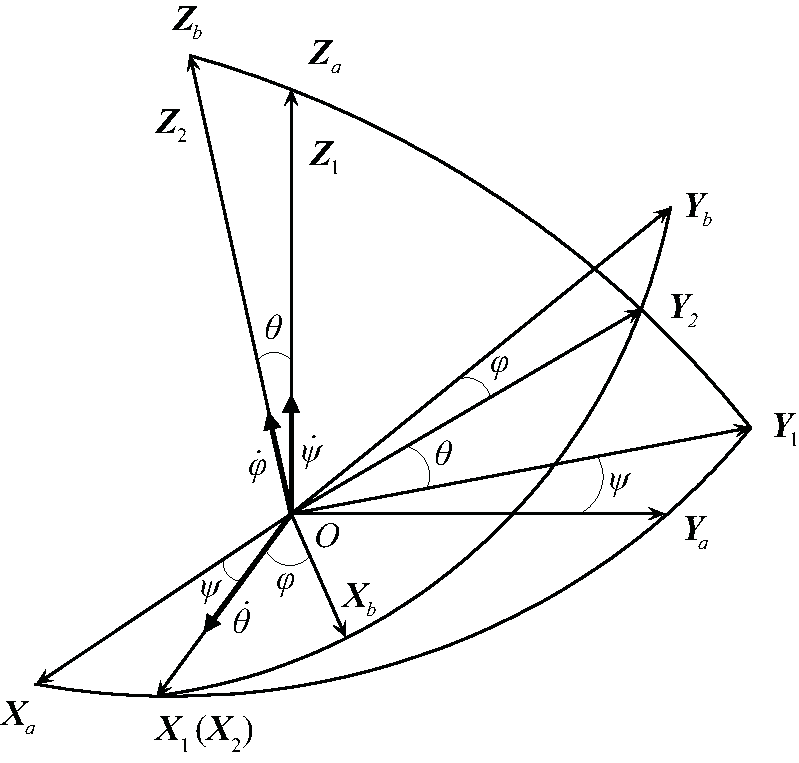
\includegraphics[width=0.8\linewidth]{pic/ZXZ}
		\caption{$ZXZ$顺序欧拉角旋转}
		\label{ZXZ}
	\end{minipage}
	\begin{minipage}{0.5\linewidth}
		\centering
		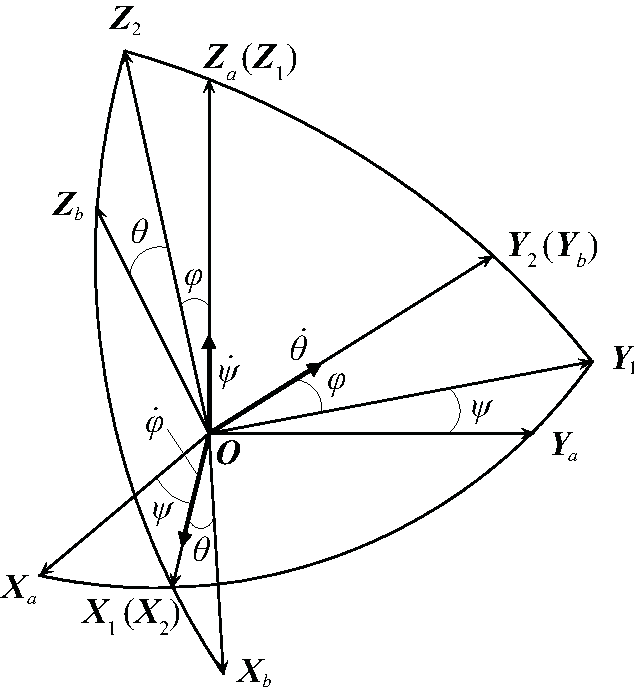
\includegraphics[width=0.695\linewidth]{pic/ZXY}
		\caption{$ZXY$顺序欧拉角旋转}
		\label{ZXY}
	\end{minipage}
\end{figure}
由公式 \eqref{eq:zxz} 可知,若欧拉角$\theta = 0\degree$,则欧拉转动处于奇异状态,欧拉角$\psi, \varphi$不能唯一确定。因此,$\theta$的取值范围为$0\degree<\theta<180\degree$。
\vspace*{1em}

\sssection[$ZXY$旋转顺序]

如图 \ref{ZXY} 所示,方向余弦矩阵和$ZXY$顺序欧拉角的关系
\begin{equation}
	\bm{C}_{ba} = \bm{C}_y(\theta)\bm{C}_x(\varphi)\bm{C_z(\psi)} =
	\begin{bmatrix}
		\cos \theta \cos \psi - \sin \varphi \sin \theta \sin \psi & \cos \theta \sin \psi + \sin \varphi \sin \theta \cos \psi & -\cos \varphi \sin \theta \\
		-\cos \varphi \sin \psi & \cos \varphi \cos \psi & \sin \varphi \\
		\sin \theta \cos \varphi + \sin \varphi \cos \theta \sin \psi & \sin \theta \sin \psi - \sin \varphi \cos \theta \cos \psi & \cos \varphi \cos \theta 
	\end{bmatrix}
\end{equation}
通过与方向余弦矩阵的对应项进行对比,可以计算得到
\begin{equation}
	\begin{cases}
		\, \psi = -\tan^{-1}\left( \dfrac{C_{21}}{C_{22}} \right) \\
		\, \theta = \sin^{-1}\big( C_{23} \big) \\
		\, \varphi = \tan^{-1} \left( \dfrac{C_{13}}{C_{33}} \right)
	\end{cases}
	\label{eq:zxy}
\end{equation}

由公式 \eqref{eq:zxy} 可知,若欧拉角$\theta = \pm 90 \degree$,则欧拉转动处于奇异状态,欧拉角$\psi, \varphi$在同一平面转动,不能唯一确定。
\vspace*{0.5em}



\subsection{欧拉轴角}
\vspace*{-1.5em}

\defination[欧拉轴 / 角]
{
	坐标系$S_b$相对坐标系$S_a$的姿态参数可以用单位矢量$\bm{e}$在参考坐标系$S_a$的三个分量$e_x, e_y, e_z$以及绕此转轴的转角$\varPhi$这4个参数来描述,称为\dy[欧拉轴 / 角]{OLZJ}参数。矢量$\bm{e}$称为\dy[欧拉轴]{OLZ},$\varPhi$称为\dy[欧拉转角]{OLZJ}。
}

\sssection[欧拉轴 / 角求方向余项矩阵]

方向余项矩阵$\bm{C}_{ba}$可由欧拉轴 / 角参数$\bm{e}, \varPhi$得到,即
\begin{align}
	\bm{C}_{ba} 
	& = \cos \varPhi \bm{E}_e + \big( 1 - \cos \varPhi \big) \bm{e} \bm{e}^{\text{T}} - \sin \varPhi \bm{e}^{\times} \notag \\
	& = 
	\begin{bmatrix}
		\cos \varPhi + e_x^2 \big( 1 - \cos \varPhi \big) & e_x e_y \big( 1 - \cos \varPhi \big) + e_z \sin \varPhi & e_x e_z \big( 1 - \cos \varPhi \big) - e_y \sin \varPhi \\
		e_x e_y \big( 1 - \cos \varPhi \big) - e_z \sin \varPhi & \cos \varPhi + e_y^2 \big( 1 - \cos \varPhi \big) & e_y e_z \big(1 - \cos \varPhi \big) + e_x \sin \varPhi \\
		e_x e_z \big( 1 - \cos \varPhi \big) + e_y \sin \varPhi & e_y e_z \big( 1- \cos \varPhi \big) - e_x \sin \varPhi & \cos \varPhi + e_z^2 \big( 1- \cos \varPhi \big)
	\end{bmatrix}
\end{align}
\clearpage
\vspace*{-2.5em}

\proof 如图 \ref{欧拉轴角} 所示,设矢量$\bm{a}$是固定在坐标系$S_a$的任意矢量,矢量$\bm{b}$是固定于坐标系$S_b$中的矢量。在绕欧拉轴$\bm{e}$旋转前,坐标系$S_a$和$S_b$重合,此时矢量$\bm{a} = \bm{b}$。设矢量$\bm{a}$与欧拉轴$\bm{e}$成$\theta$角,当绕$\bm{e}$轴旋转$\varPhi$角时,矢量$\bm{b}$在轴线为$\bm{e}$的圆锥面上扫过,且与$\bm{e}$的夹角不变。

\begin{figure}[!htb]
	\centering
	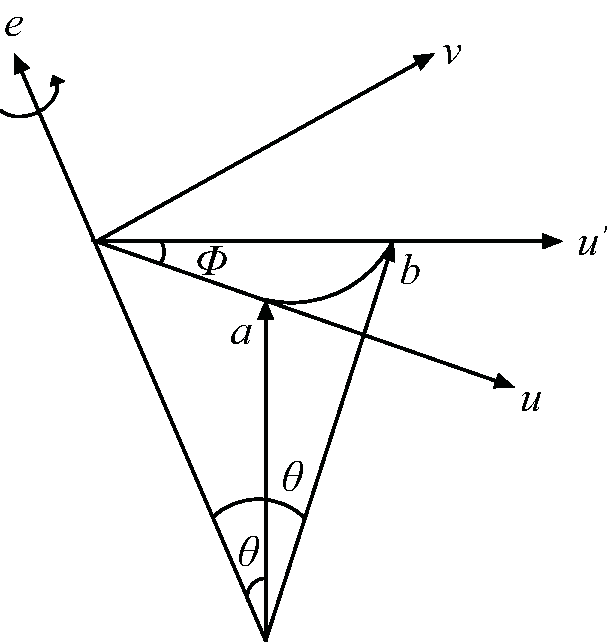
\includegraphics[width=0.28\linewidth]{pic/欧拉轴角}
	\caption{欧拉轴 / 角的坐标变换图}
	\label{欧拉轴角}
\end{figure}

\noindent 在垂直于$\bm{e}$的圆锥底面上定义矢量$\bm{u}, \bm{v}$
\begin{align*}
	\bm{v} & = \dfrac{\bm{e} \times \bm{a}}{\big| \bm{e} \times \bm{a} \big|} = \dfrac{1}{a \sin \theta}(\bm{e} \times \bm{a}) \\
	\bm{u} & = \bm{v} \times \bm{e} = \dfrac{1}{a \sin \theta} (\bm{e} \times \bm{a}) \times \bm{e} = \dfrac{1}{a \sin \theta}\big[ \bm{a} - (\bm{e} \cdot \bm{a})\bm{e} \big] 
\end{align*}
过矢量$\bm{b}$的端点,作矢量$\bm{u}'$,即
\begin{equation*}
	\bm{u}' = \cos \varPhi \bm{u} + \sin \varPhi \bm{v}
\end{equation*}
将矢量$\bm{a}, \bm{b}$用上面的矢量表示为
\begin{align}
	\bm{a} & = a \big( \cos \theta \bm{e} + \sin \theta \bm{u} \big) \\
	\bm{b} & = a \big( \cos \theta \bm{e} + \sin \theta \bm{u}' \big)
\end{align}
消去$\bm{u}, \bm{u}'$,可以得到
\begin{equation}
	\bm{b} = \cos \varPhi \bm{a} + ( 1 - \cos \varPhi ) (\bm{e} \cdot \bm{a})\bm{e} + \sin \varPhi(\bm{e} \times \bm{a})
\end{equation}
分别取$\bm{a} = \bm{i}_a, \bm{j}_a, \bm{k}_a; \bm{b} = \bm{i}_b, \bm{j}_b, \bm{k}_b$,可以得到
\begin{equation}
	\begin{cases}
		\, \bm{i}_b = \cos \varPhi \bm{i}_a+ ( 1 - \cos \varPhi ) (\bm{e} \cdot \bm{i}_a)\bm{e} + \sin \varPhi(\bm{e} \times \bm{i}_a) \\
		\, \bm{j}_b = \cos \varPhi \bm{j}_a+ ( 1 - \cos \varPhi ) (\bm{e} \cdot \bm{j}_a)\bm{e} + \sin \varPhi(\bm{e} \times \bm{j}_a) \\
		\, \bm{k}_b = \cos \varPhi \bm{k}_a+ ( 1 - \cos \varPhi ) (\bm{e} \cdot \bm{k}_a)\bm{e} + \sin \varPhi(\bm{e} \times \bm{k}_a)
	\end{cases}
	\label{eq:zj}
\end{equation}
将$\bm{e}$在坐标系$S_a$中分解为$\bm{e} = e_x \bm{i}_a + e_y \bm{j}_a + e_z \bm{k}_a $,代入公式 \eqref{eq:zj} 合并即可。
\vspace*{1em}


\sssection[由方向余弦矩阵确定欧拉轴 / 角参数]

若已知方向余弦矩阵$\bm{C}_{ba}$,可以计算得到欧拉轴 / 角参数,得
\begin{align}
	\cos \varPhi = \dfrac{\text{tr} \bm{C}_{ba} - 1}{2} \\
	\bm{e} = \dfrac{1}{2 \sin \varPhi} 
	\begin{bmatrix}
		C_{23} - C_{32} \\
		C_{31} - C_{13} \\
		C_{12} - C_{21}
	\end{bmatrix}
\end{align}
其中,$\text{tr} \bm{C}_{ba}$是方向余弦矩阵的迹,$\text{tr} \bm{C}_{ba} = C_{11} + C_{12} + C_{13}$。绕任意轴转动相同的$\varPhi$角,方向余项矩阵的迹不变。
\clearpage

\noindent 将公式展开,对应得到以下3组解:

\noa[1] 当$\text{tr} \bm{C}_{ba} \neq 3, -1$时,可以直接计算分量$e_x, e_y, e_z$。

\noa[2] 当$\text{tr} \bm{C}_{ba} = 3$时,此时对应转角$\varPhi = 0, \pm 2 \pi, \pm 4 \pi, \cdots$,方向余弦矩阵$\bm{C}_{ba}$为单位矩阵,$e_x, e_y, e_z$无法确定。这种情况相当于没有发生转动。

\noa[3] 当$\text{tr} \bm{C}_{ba} = -1$时,对应转角$\varPhi = \pm \pi, \pm 3 \pi, \pm 5 \pi, \cdots$,此时$\bm{C}_{ba} = 2 \bm{e}\bm{e}^{\text{T}} - \bm{E}_3$,则有
\begin{equation}
	\begin{cases}
		\, e_x = \pm \sqrt{\dfrac{1 + C_{11}}{2}}, \qquad e_y = \pm \sqrt{\dfrac{1+ C_{22}}{2}}, \qquad e_z = \pm \sqrt{\dfrac{1 + C_{33}}{2}} \\[0.5em]
		\, e_x e_y = \dfrac{1}{2} C_{12}, \hspace*{3.7em} e_ye_z = \dfrac{1}{2}C_{23}, \hspace*{3.7em} e_ze_x = \dfrac{1}{2} C_{31}
	\end{cases}
\end{equation}
其中,使用后三个方程来判断前三个方程的符号。

\begin{figure}[!htb]
	\centering
	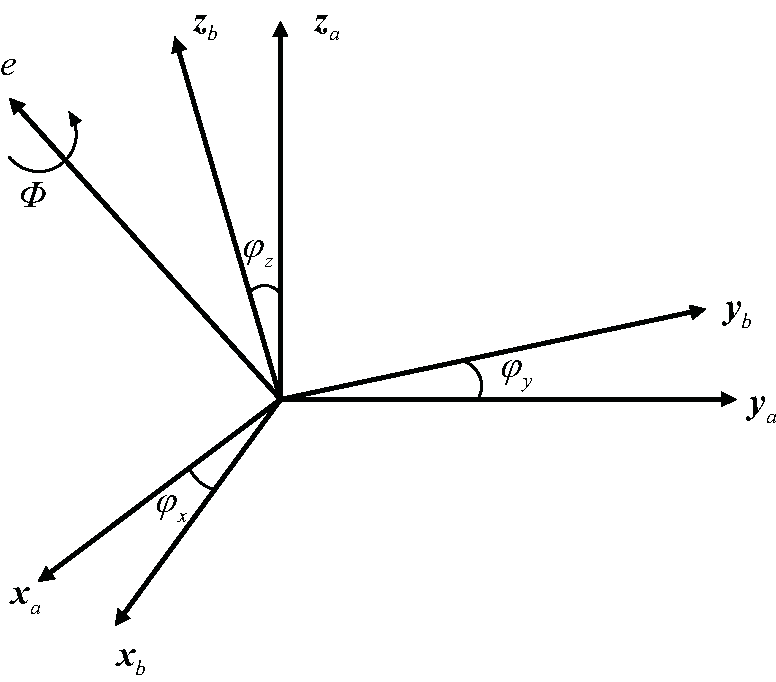
\includegraphics[width=0.4\linewidth]{pic/欧拉轴角变换}
	\vspace*{-1em}
	\caption{欧拉转角与两个坐标系之间的几何关系}
	\label{欧拉转角变换}
\end{figure}


\sssection[欧拉转角的几何意义]

如图 \ref{欧拉转角变换} 所示,令$\varphi_x, \varphi_y, \varphi_z$分别为两个坐标系对应轴之间的夹角,方向余弦矩阵的对焦线上的元素即为这几个角的余弦值,所以
\begin{equation}
	2 \cos \varPhi = \text{tr} \bm{C}_{ba} - 1 = \cos \varphi_x + \cos \varphi_y + \cos \varphi_z - 1
\end{equation}
利用半角公式$\cos \alpha = 1 - 2 \sin^2 \dfrac{\alpha}{2}$,则
\begin{equation}
	\sin^2 \dfrac{\varPhi}{2} = \dfrac{1}{2} \left( \sin^2 \dfrac{\varphi_x}{2} + \sin^2 \dfrac{\varphi_y}{2} + \sin^2 \dfrac{\varphi_z}{2} \right)
\end{equation}

当偏角较小时,有
\begin{equation}
	\varPhi \approx \dfrac{\sqrt{2}}{2} \sqrt{\varphi_x^2 + \varphi_y^2 + \varphi_z^2}
\end{equation}
这个公式对于评价旋转误差是很有用的。





















